%%%%%%%%%%%%%%%%%%%%%%%%%%%%%%%%%%%%
% Don't touch these options
%%%%%%%%%%%%%%%%%%%%%%%%%%%%%%%%%%%%


\documentclass[english, 11pt]{article}\usepackage[]{graphicx}\usepackage[]{color}
%% maxwidth is the original width if it is less than linewidth
%% otherwise use linewidth (to make sure the graphics do not exceed the margin)
\makeatletter
\def\maxwidth{ %
  \ifdim\Gin@nat@width>\linewidth
    \linewidth
  \else
    \Gin@nat@width
  \fi
}
\makeatother

\definecolor{fgcolor}{rgb}{0.345, 0.345, 0.345}
\newcommand{\hlnum}[1]{\textcolor[rgb]{0.686,0.059,0.569}{#1}}%
\newcommand{\hlstr}[1]{\textcolor[rgb]{0.192,0.494,0.8}{#1}}%
\newcommand{\hlcom}[1]{\textcolor[rgb]{0.678,0.584,0.686}{\textit{#1}}}%
\newcommand{\hlopt}[1]{\textcolor[rgb]{0,0,0}{#1}}%
\newcommand{\hlstd}[1]{\textcolor[rgb]{0.345,0.345,0.345}{#1}}%
\newcommand{\hlkwa}[1]{\textcolor[rgb]{0.161,0.373,0.58}{\textbf{#1}}}%
\newcommand{\hlkwb}[1]{\textcolor[rgb]{0.69,0.353,0.396}{#1}}%
\newcommand{\hlkwc}[1]{\textcolor[rgb]{0.333,0.667,0.333}{#1}}%
\newcommand{\hlkwd}[1]{\textcolor[rgb]{0.737,0.353,0.396}{\textbf{#1}}}%
\let\hlipl\hlkwb

\usepackage{framed}
\makeatletter
\newenvironment{kframe}{%
 \def\at@end@of@kframe{}%
 \ifinner\ifhmode%
  \def\at@end@of@kframe{\end{minipage}}%
  \begin{minipage}{\columnwidth}%
 \fi\fi%
 \def\FrameCommand##1{\hskip\@totalleftmargin \hskip-\fboxsep
 \colorbox{shadecolor}{##1}\hskip-\fboxsep
     % There is no \\@totalrightmargin, so:
     \hskip-\linewidth \hskip-\@totalleftmargin \hskip\columnwidth}%
 \MakeFramed {\advance\hsize-\width
   \@totalleftmargin\z@ \linewidth\hsize
   \@setminipage}}%
 {\par\unskip\endMakeFramed%
 \at@end@of@kframe}
\makeatother

\definecolor{shadecolor}{rgb}{.97, .97, .97}
\definecolor{messagecolor}{rgb}{0, 0, 0}
\definecolor{warningcolor}{rgb}{1, 0, 1}
\definecolor{errorcolor}{rgb}{1, 0, 0}
\newenvironment{knitrout}{}{} % an empty environment to be redefined in TeX

\usepackage{alltt}
\usepackage[T1]{fontenc}
%\usepackage[latin9]{inputenc}
\usepackage{geometry}
\geometry{verbose,tmargin=2.5cm,bmargin=2.5cm,lmargin=2.5cm,rmargin=2.5cm}
\usepackage{float}
\usepackage{graphicx}
\usepackage{babel}
\usepackage{hyperref}
\usepackage{bm}
\usepackage[T1]{fontenc}
\IfFileExists{upquote.sty}{\usepackage{upquote}}{}
\begin{document}

%%%%%%%%%%%%%%%%%%%%%%%%%%%%%%%%%%%%
% Title Page
%%%%%%%%%%%%%%%%%%%%%%%%%%%%%%%%%%%%
\title{Unsupervised Learning of Cellular Development Time}


\author{Caleb Lareau}


\date{11 May 2017}
\maketitle
\begin{abstract}
\noindent Recent advances in microfluidic technologies have enabled an unprecedented characterization of epigenomic and transcriptomic profiles of single cells. Though the dimension of the single cell feature space often exceeds 20,000, a commonly desired yet unobserved variable associated with cellular development time must be estimated using computational methods. Herein, I motivate the identification of this latent dimension termed \textit{pseudotime} and contextualize its inference as an application of unsupervised learning. Moreover, I present the statistical basis of both linear (principal component analysis; PCA) and non-linear (Gaussian process latent variable modeling; GPLVM) dimension reduction from a probabilistic perspective. To evaluate the performance of the methods of unsupervised learning in this context, I examine the inferred pseudotime against the true developmental ordering of murine embryonic stem cell development. 

\newpage{}
\end{abstract}

%%%%%%%%%%%%%%%%%%%%%%%%%%%%%%%%%%%%
% End Title Page
%%%%%%%%%%%%%%%%%%%%%%%%%%%%%%%%%%%%




%%%%%%%%%%%%%%%%%%%%%%%%%%%%%%%%%%%%
\section{Introduction}
wherein the couple has already pledged over \$50 million to profile an estimated 35 trillion cells from various stages of human development. \cite{HCA}

The establishment of biomarkers related to early versus late development in hematopoesis acute myeloid leukemia (AML). \cite{corces2016lineage} 

Recently reviewed in \cite{cannoodt2016computational}

single cell heme atac \cite{buenrostro2017single}

PCA \cite{jolliffe2002principal}

pPCA \cite{tipping1999probabilistic}

In the 1940s and 1950s, Whittle\cite{whittle1952principal} and Young \cite{young1941maximum} provided a likelihood-based framework that enabled the derivations of principal components using a factor analysis framework. Notably, this likelihood-based framework enabled a probablistic interpretation of PCA, enabling uncertainty in both the components and the loadings to be estimated from a posterior distribution. 

\begin{figure}[H]
\begin{center}
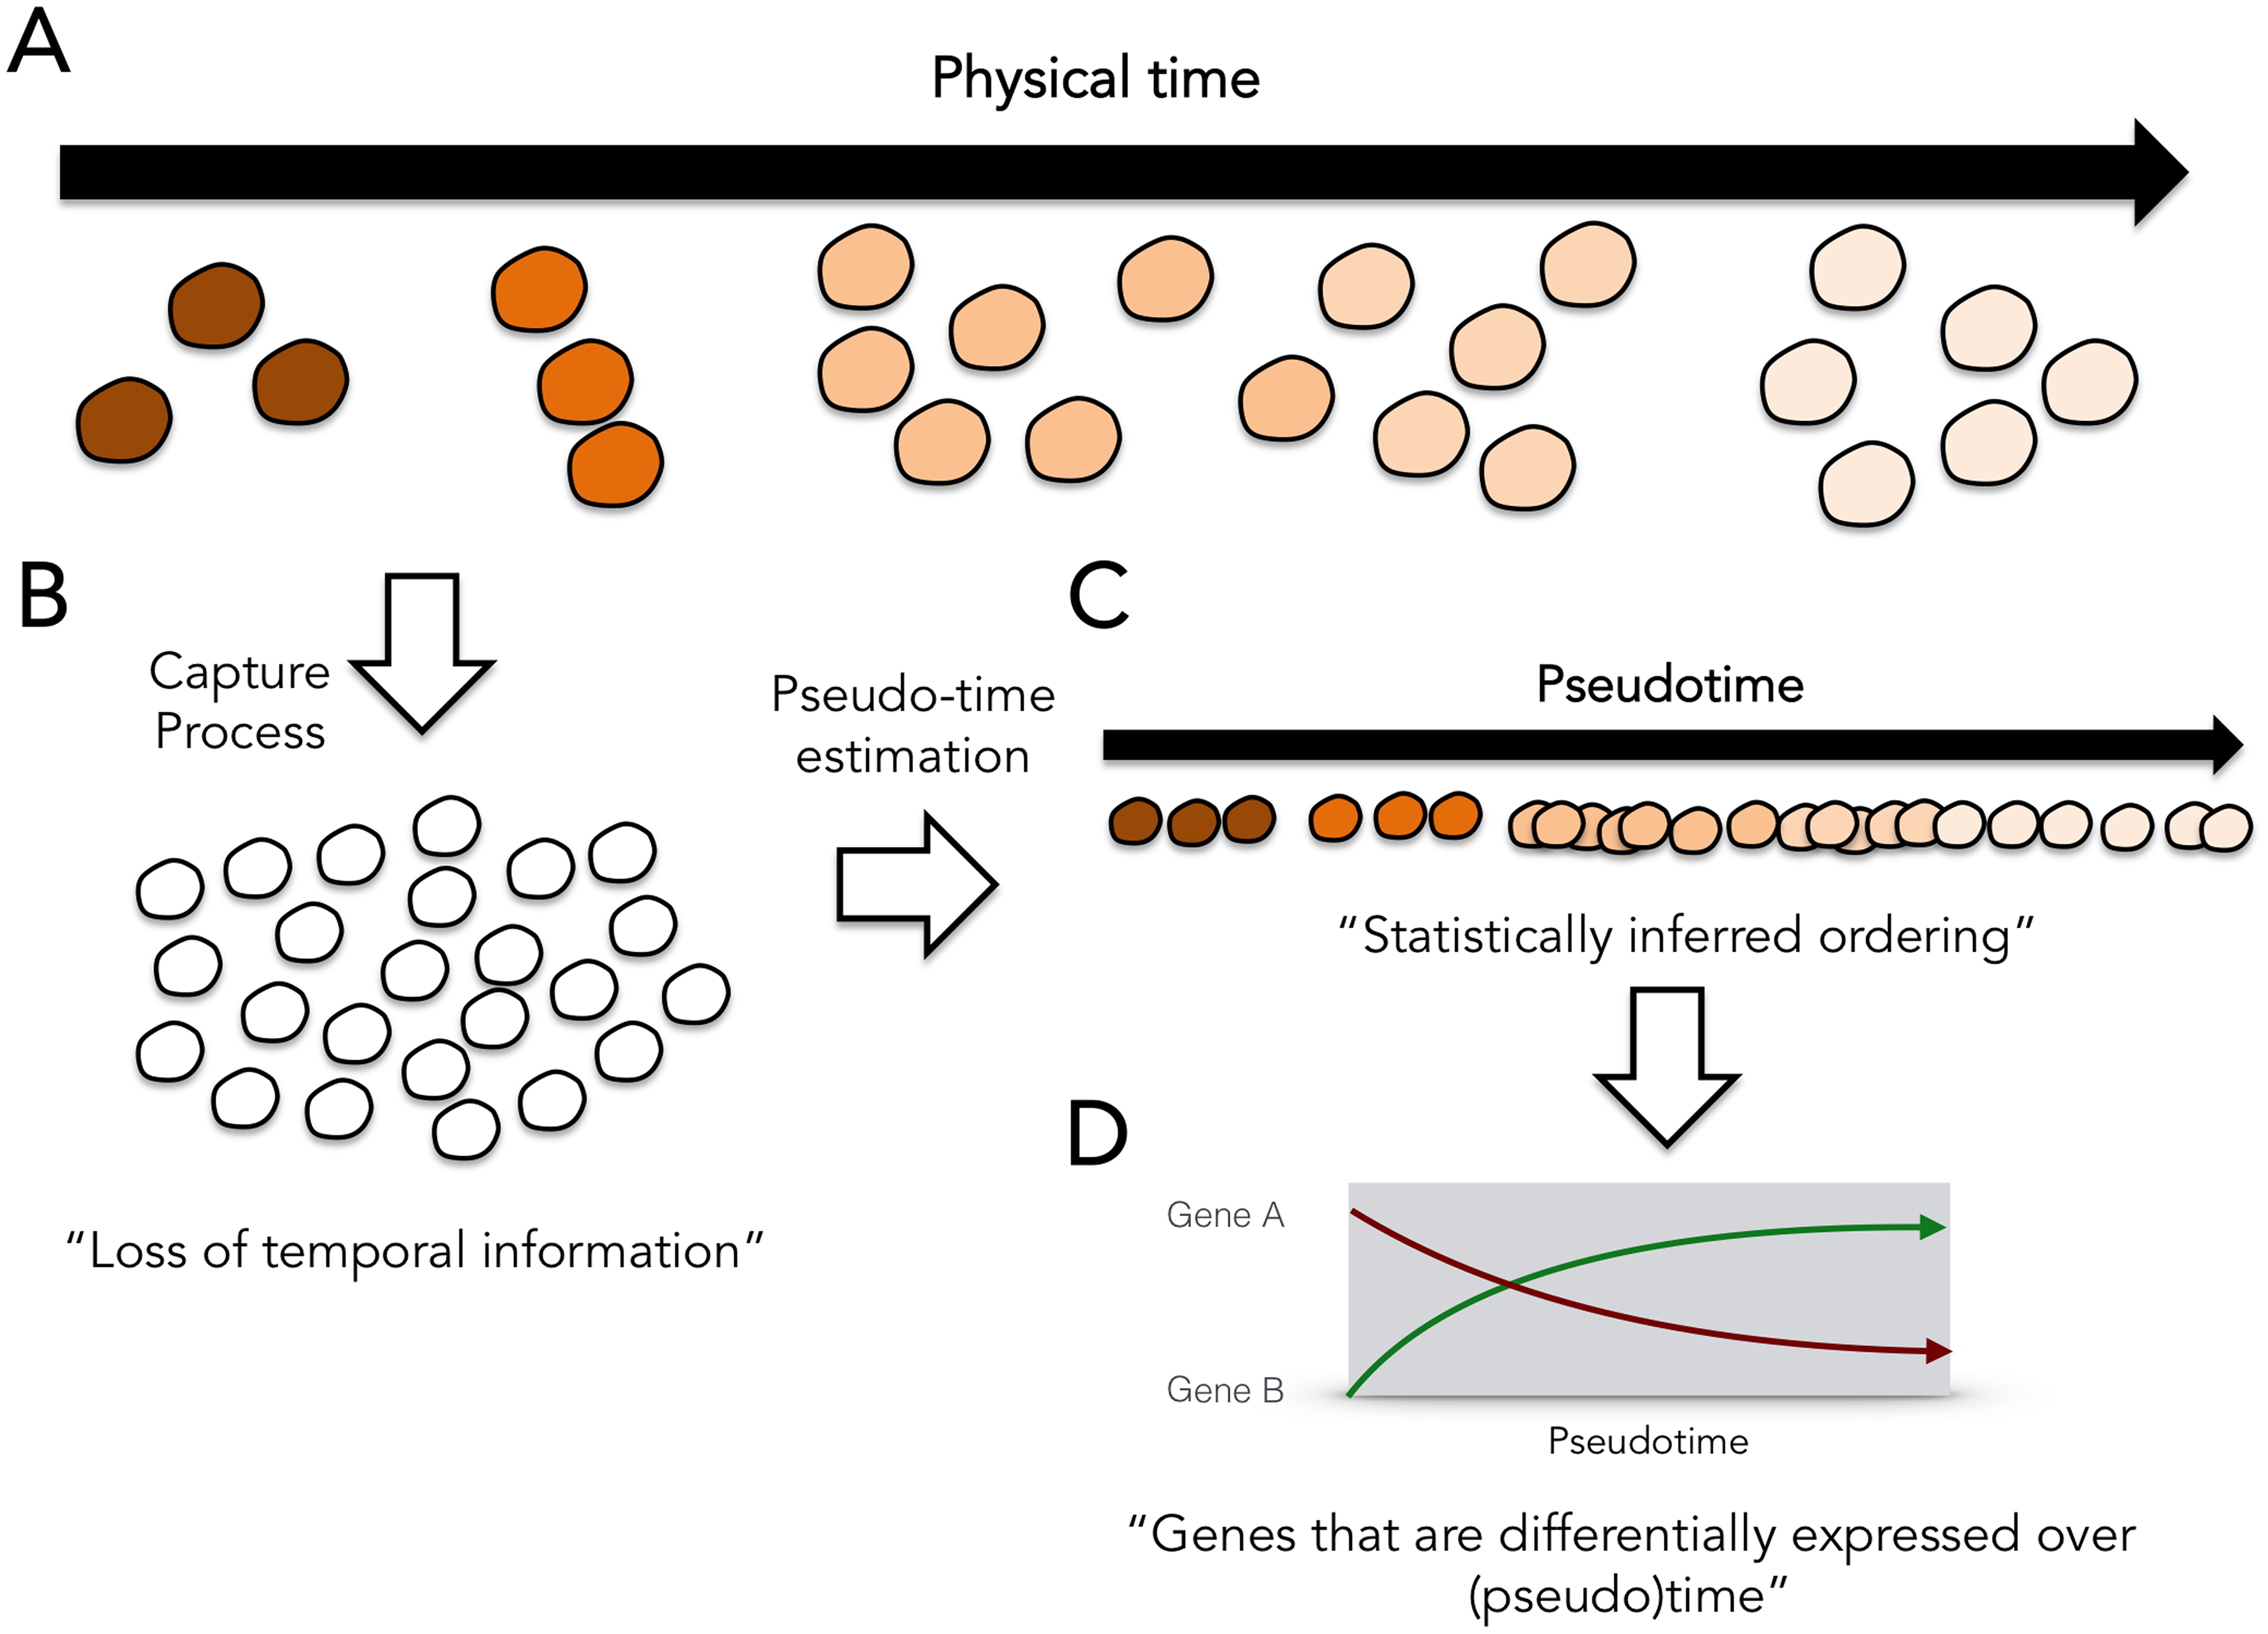
\includegraphics[scale=1.0]{images/fig1campbell.png}
\end{center}
\caption{\textbf{Overview of single-cell sample collection and developmental ordering.} (A) For a set of cells (each single cell is indicated by a circle), a true developmental time associated with its development is a latent variable (indicated by the color gradient) that accounts for some variance in the transcriptomic profiles. (B) While this developmental time is a true feature of these cells, current technologies do not allow for the capture of this physical/developmental time ordering. (C) Thus, computational and statistical approaches are required to approximate the developmental time. This approximation is referred to as \textit{pseudotime}. (D) . Image reproduced without permission from \cite{campbell2016order}. }
\end{figure}


\subsection{Subsection }

If you don't need subsections or would prefer to organize your paragraphs
in another way, feel free to go without.




%%%%%%%%%%%%%%%%%%%%%%%%%%%%%%%%%%%%
\section{Setting}

Introduce your notation and clearly define your assumptions. 

\begin{figure}[H]
\begin{center}
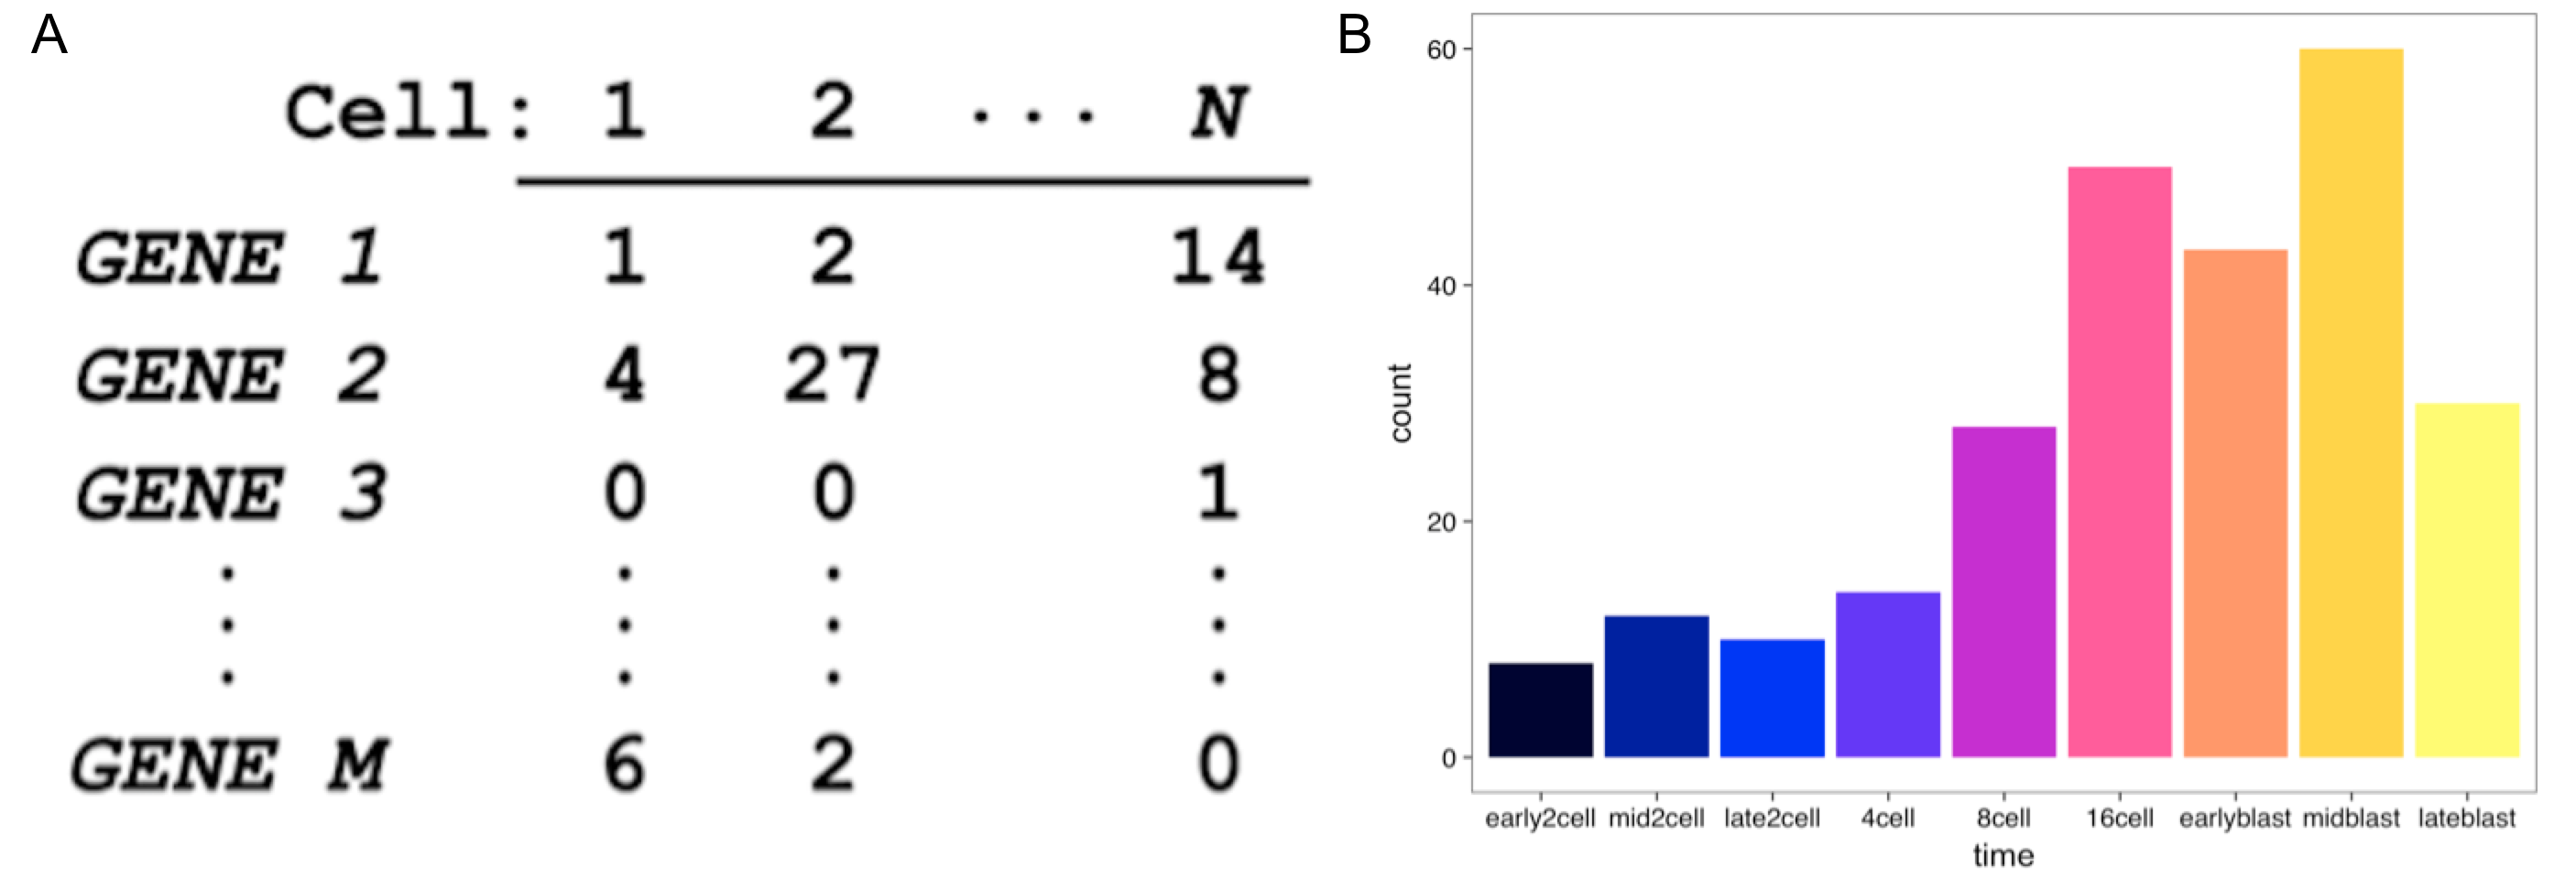
\includegraphics[scale=0.3]{images/Figure2.png}
\end{center}
\caption{\textbf{Data summary for single cell analysis setting.} (A) An example of a ``perfect" latent dimension (x-axis) where the true ordering of the nine embryonic states (y-axis) is inferred. (B) The comparison of the true developmental ordering (y-axis) against a linear unsupervised learning dimension (principal component 1), indicating a modest}
\end{figure}





%%%%%%%%%%%%%%%%%%%%%%%%%%%%%%%%%%%%
\section{Methods}

Present the statistical methods.

\subsection{Principal component analysis}
$\mathbf{Y}$ is a $D$ x $n$ matrix. Compute the covariance matrix--

$$ \mathbf{\Sigma} = E(\mathbf{YY^{T}}) - \mathbf{\mu \mu^T}$$
where $\mathbf{\mu} = E(\mathbf{Y})$ <br>

Then compute the spectral decomposition of $\mathbf{\Sigma}$

$$\mathbf{\Sigma} a_j = \lambda_j a_j$$
for $j \in (1, ..., D)$
<br><br>
Then $a_j$ represent the eigenvectors of the data matrix $\mathbf{Y}$. <br> Note the ordering of $j$ is meaningful-- 
$$ \lambda_1 \geq \lambda_2 \geq ... \geq \lambda_D \geq 0$$


\subsection{Factor analysis}

$\mathbf{Y}$ is a $D$ x $n$ matrix. $\mathbf{x}$ is a $d$ x $n$ matrix ($d < D$). Want to relate $\mathbf{x}$ and $\mathbf{Y}$ and assume that the relationship is linear--

$$ \mathbf{Y = Wx} + \epsilon$$<br>
where $W$ is a $D$ x $d$ matrix. <br><br>

By convention (after locating the matrix),<br><br> $$\mathbf{x} \sim \mathcal{N} (0, \mathbf{I})$$<br>
where $\mathbf{I}$ is the identity matrix of dimension $d$ x $d$. 

\subsection{Probablistic PCA}

$\psi_i$ element of the diagonal of $\Psi$; add constraint $\psi_i = \sigma^2$<br><br>
Assume $\sigma^2$ known, MLE yields same $W$ as PCA <br><br>
$$  \mathcal{L} = \frac{-N}{2}\{ D\log(2\pi) + \log|\mathbf{C}| + \textrm{tr}(\mathbf{C}^{-1}\mathbf{\Sigma})  \}   $$<br>
$$\mathbf{C} = \mathbf{WW^T }+ \mathbf{\Psi} $$ <br>
$$  \mathbf{x} = \mathbf{C^{-1}W^{T}Y}$$

Probablistic PCA (Tipping and Bishop)
- Assuming $\sigma^2$ may not be reasonable; want to estimate it from the data (keep in likelihood)
- Can estimate $\mathbf{W}, \sigma^2$ using EM and with a prior over $\mathbf{x}$

For  $\mathbf{W_{\textrm{MLE}}}$, <br><br> $$\sigma_{MLE}^2 = \frac{1}{D-d} \sum_{j = d +1}^D \lambda_j $$

- Similarly, we can integrate over $\mathbf{W}$ given a prior, yielding <br><br>
$$  \mathbf{x} \sim  \mathcal{N} (\mathbf{C^{-1}W^{T}Y}, \sigma^2C^{-1})$$ <br>


Computational methods for inferring principal components under this likelihood framework are availabel through the \texttt{pcaMethods} \texttt{R} package.

\subsection{Bayesian PCA}
Though not utilized in this particular data analysis, the derivation of probablistic PCA enables a Bayesian framework for performing linear dimensionality reduction and putting a prior on these reduced dimensions. \cite{bishop1999bayesian} Methods for computing principal components with Bayesian priors and interpretations are also accessible through the \texttt{pcaMethods} \texttt{R} package.

\subsection{Gaussian Process Latent Variable Modeling}

\begin{equation}
\mathbf{Y} \sim  \mathcal{N} (0, \mathbf{C}), \mathbf{C} = \mathbf{WW^T }+ \mathbf{\Psi}
\end{equation}

\begin{equation}
\mathbf{C}(\mathbf{W_i},\mathbf{W_j}) = \mathbf{W_i^T}\mathbf{W_j} + \sigma^2\delta_{ij}
\end{equation}

\begin{equation}
\mathbf{C}(\mathbf{W_i},\mathbf{W_j}) = \theta_{rbf} \exp \Big(\frac{-\gamma}{2}(\mathbf{W_i}-\mathbf{W_j})^{T}(\mathbf{W_i}-\mathbf{W_j})  \Big) + ...
\end{equation}


- (2) being a special case (linear, iid) of (3)
- Computationally more challenging, but there are fast algorithms out there






%%%%%%%%%%%%%%%%%%%%%%%%%%%%%%%%%%%%
\section{Data Application}
From mice \cite{deng2014single}
A small simulation study or application to existing dataset.

\begin{figure}[H]
\begin{center}
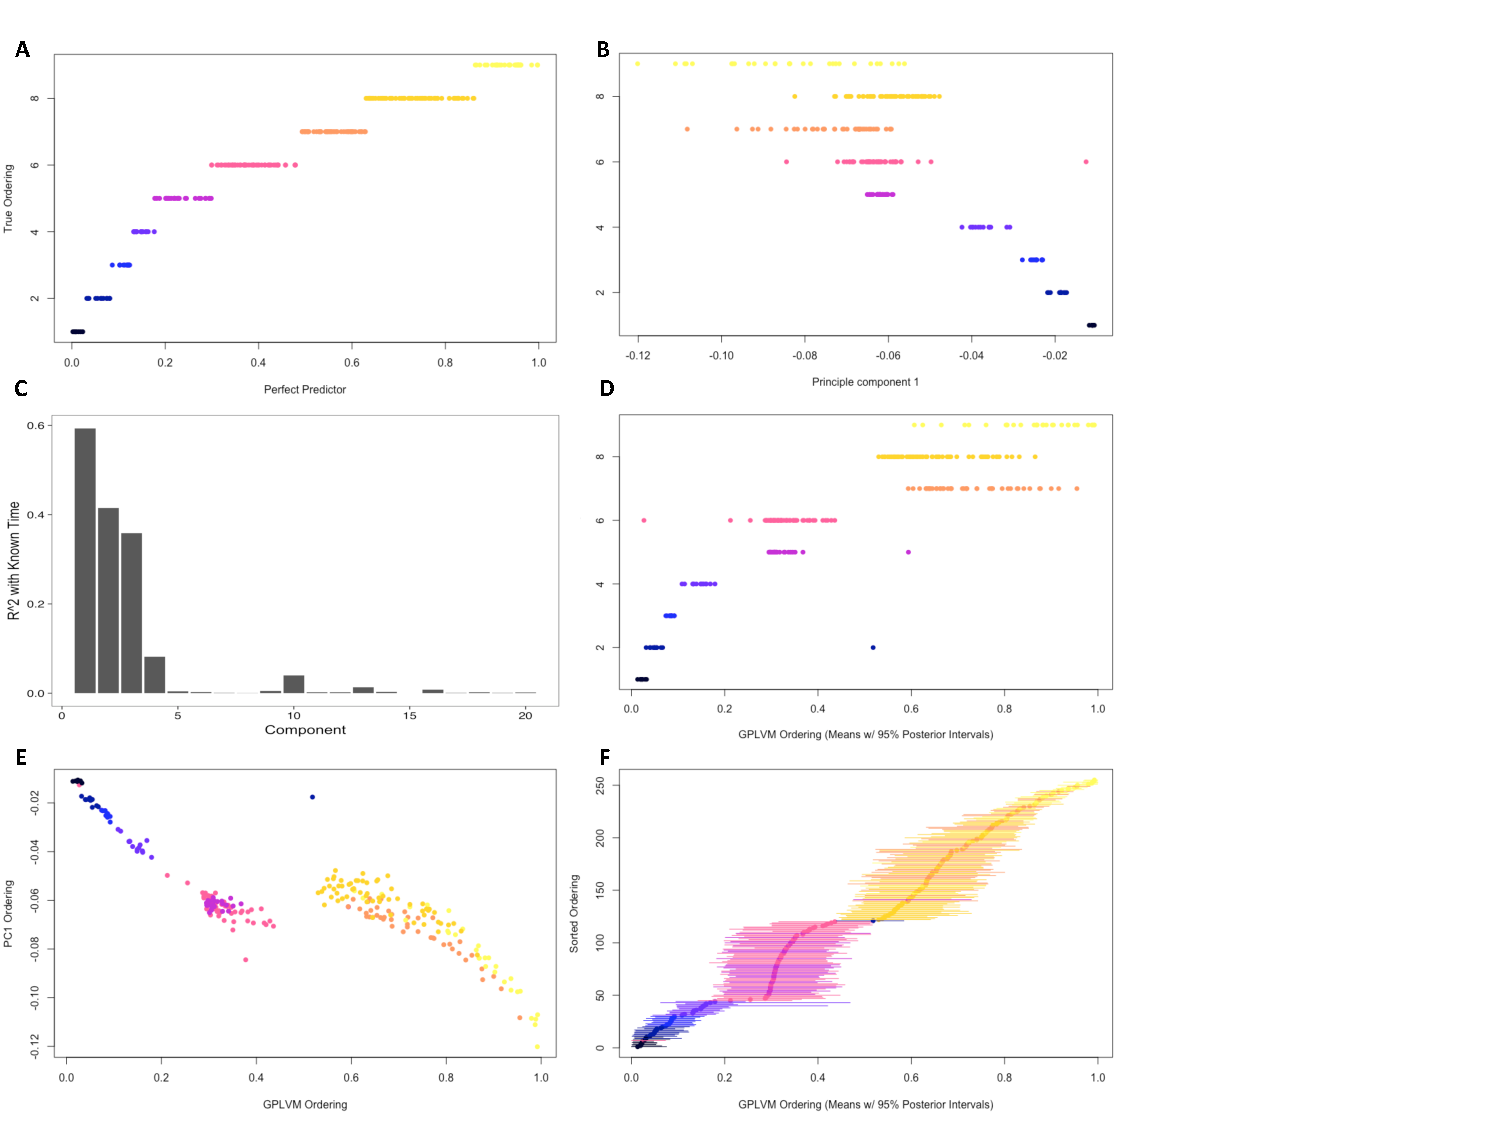
\includegraphics[scale=0.8]{images/Figure3.pdf}
\end{center}
\caption{\textbf{Summary of unsupervised learning results applied to murine embyronic stem cell development.} (A) An example of a ``perfect" latent dimension (x-axis) where the true ordering of the nine embryonic states (y-axis) is inferred ($r^2 = 0.88$). (B) The comparison of the true developmental ordering (y-axis) against a linear unsupervised learning dimension (principal component 1), indicating a decent approximation of true developmental ordering ($r^2 = 0.59$). (C) Barplot depicting the $r^2$ for the first 20 principal components similar to what was shown for PC1 in (B). This plot suggests that a non-linear dimension reduction may best approximate the true developmental ordering. (D) The comparison of the true developmental ordering (y-axis) against a non-linear unsupervised learning dimension (Gaussian Process latent variable 1), indicating a better approximation of true developmental ordering ($r^2 = 0.78$). (E) Comparison of linear (y-axis; PC1) and non-linear (x-axis; GP latent variable 1) reduced dimensions. The non-linear unsupervised learning technique separates day 8 and day 16 development from the blastocyst samples. (F) Uncertainty associated with GP latent variable 1 depicted with the 95\% posterior confidence interval. }
\end{figure}





GPLVM \cite{lawrence2004gaussian}




%%%%%%%%%%%%%%%%%%%%%%%%%%%%%%%%%%%%
\section{Conclusion}

GPLVM have recently been applied to resolve Th1/Tfh fate bifurcation in mice exposed to malaria, providing novel insights into the genetic perturbations associated with T-cell response and memory to foreign antigens. \cite{lonnberg2017single} More generally, Welch $et$ $al.$ showed that GPLVM provide a flexible means to infer development ordering in single cells using not just RNA profiles but also chromatin accessibility, methylation, and histone modifications derived from single-cell experiments. \cite{welch2017manifold}

\section*{Accessibility}

All code and data used to generate the figures, slides, and writeup are made publicly available at \url{https://github.com/caleblareau/BST245_Final}.

\newpage{}


%%%%%%%%%%%%%%%%%%%%%%%%%%%%%%%%%%%%
\bibliographystyle{ieeetr}
\bibliography{Lareau245Final}{}

\end{document}
